

\documentclass[12pt]{article}

%\pagestyle{empty} 
\usepackage{amsmath}
\usepackage{algpseudocode}
\usepackage{algorithm}
\usepackage[english]{babel}
\usepackage{amsthm}
\usepackage{amssymb}
\usepackage{color}
\usepackage{graphicx}
\usepackage{epsfig}

\newcommand{\vs}{\vspace{2mm}}
\newcommand{\ls}{\vspace{5mm}} 

\newcommand{\ms}{\vspace{3mm}}
\newcommand{\bc}{\begin{center}}
\newcommand{\ec}{\end{center}}
\newcommand{\sm}{\small}
\newcommand{\hs}{\hspace{10mm}}
\newcommand{\ha}{\hspace{1mm}}
\newcommand{\bo}{\rule{2mm}{3mm}}
\textheight=680pt
\textwidth=460pt
\hoffset=-50pt
\voffset=-50pt
%\topmargin=-0.5in
%\textheight=10in
%\oddsidemargin=0.125in
%\evensidemargin=0.125in
%\textwidth=7.5in
\begin{document}
\bc\ { \bf  Homework  1 (50 points)}  Due: September 13, 2024 11:59 pm\\

 { \bf COMPSCI 733: Advanced Algorithms and Designs } \ec\ 
\ls\

\noindent{\bf Documentation:} (5 points)
Type your solutions using Latex \\
(www.overleaf.com or https://www.latex-project.org/ ). Submit your solutions (pdf is enough)  to Canvas. 




\vs\

\noindent{\bf Problem 1: (15 points)}
Assume we have a one dimensional array of real numbers with $A.length = n$ and indices, $1, 2, \ldots, n$.
In the code for InsertionSort  shown below, the outer loop index $j$ goes from 2 to $n$, and the inner index i of the while loop goes “backward”. 

\begin{algorithm}
\caption{INSERTION-SORT-FORWARD(A)}
\begin{algorithmic}[1]
\For {$j=2$ to $n$}
\State{$key=A[j]$}
\State{//Insert $A[j]$ into the sorted sequence $A[1,\ldots,j-1].$}
\State{$i=j-1$}
\While{$i > 0$ and $A[i] > key$} 
  State{$A[i+1]=A[i]$} 
    \State $i = i-1$
\EndWhile
\State {$A[i+1] = key$}
\EndFor
\end{algorithmic}
\end{algorithm}

\begin{itemize}
 \item[(a)] Write a version of the pseusocode for InsertionSortBackward where the outer index j goes “backward”, and the inner index i goes “forward”.  

\begin{algorithm}
\caption{INSERTION-SORT-BACKWARD(A)}
\begin{algorithmic}[1]
\State{Your pseudocode goes here.}
\end{algorithmic}
\end{algorithm}

\item[(b)] Prove that your program (InsertionSortBackward)is correct.
See CLRS Chapter 2 and the given "ProgramCorrectness.pptx" slides.

Steps:
\begin{itemize}
\item[1.]	 Write a loop invariant.
\item[2.]	Show Initialization holds.
\item[3.]Show Maintenance  holds.
\item[4.]	Show Termination holds.
\end{itemize}
\end{itemize}

\vs\
\pagebreak

\noindent{\bf Problem 2: (15 points) }

A tree is a simple connected graph with no cycles.

\begin{figure}[!h]
\centering
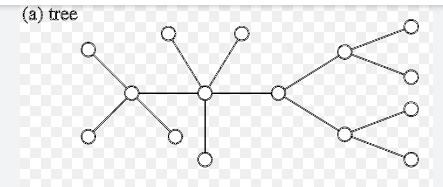
\includegraphics[scale=1]{TreeExample.jpg}
\caption{}
\label{fig1}
\end{figure}

	Use the mathematical induction steps given  in the following template to prove that a tree with $n$ vertices has exactly $n-1$ edges for all $n \geq 1$.
\vs\

\noindent{\bf Induction proof template:}

\noindent{$P(n):$}   A tree with $n$ vertices has exactly $n-1$ edges.
\ls\

\noindent{\em Prove:} $P(n)$ is true for all $n \geq 1$.
\vs\

\begin{proof} (By induction on $n$)

    \begin{itemize}
    \item Prove the base case.
    \item Write the inductive hypothesis ($n=k$).
    \item Prove the inductive step. (Hint: Start with any tree with $n= k+1$ vertices.)
    \item Conclusion. (Given)
    Therefore, by the principle of mathematical induction, $P(n)$ is true for all $n \geq 1.$
    \end{itemize}
    
\end{proof}

\noindent{\bf Problem 3: (15 points)}

Use strong induction to show that every positive integer $n$ can be written as a sum of distinct powers of two, that is, as a sum of a subset of the integers $2^0 , 2^1 , 2^2 …,$ and so on  i.e., $1=2^0 , 2=  2^1 , 3=2^0+ 2^1, 4=2^2 , ... $. [Hint: For the inductive step, separately consider the cases where $k + 1$ is even and where $k+1$ is odd. When it is even, note that $(k + 1)/2$ is an integer.]
\vs\

\noindent{\bf Strong induction proof template:}

\noindent{$P(n):$}  Every positive integer $n$ can be written as a sum of distinct powers of two.
\ls\

\noindent{\em Prove:} $P(n)$ is true for all $n \geq 1$.
\vs\

\begin{proof} (By strong induction on $n$)

    \begin{itemize}
    \item Prove the base case.
    \item Write the strong inductive hypothesis ($n=1, 2, \ldots, k$).
    \item Prove the inductive step.[Hint:Separately consider the cases where $k + 1$ is even and where $k+1$ is odd. When it is even, note that $(k + 1)/2$ is an integer.] 
    \item Write the conclusion. 
    \end{itemize}
    
\end{proof}




\end{document}




